% Niveau :      PCSI *
% Discipline :  Chimie Orga I
% Mots clés :   Spectrométrie UV-visible, Réactions acidobasiques

\begin{exercise}{Parahélium et orthohélium}{3}{PCSI}
{Atomistique,Classification périodique, Structure électronique}{bermu}



\begin{questions}
    \questioncours Quantification de l'énergie dans l'atome d'hydrogène. Nombres quantiques.

\begin{EnvUplevel}
On appelle parahélium et orthohélium les deux variantes de l'atome d'hélium dans lesquelles les spins des électrons sont parallèles ou antiparallèles.
 
    \begin{figure}[H]
        \centering
        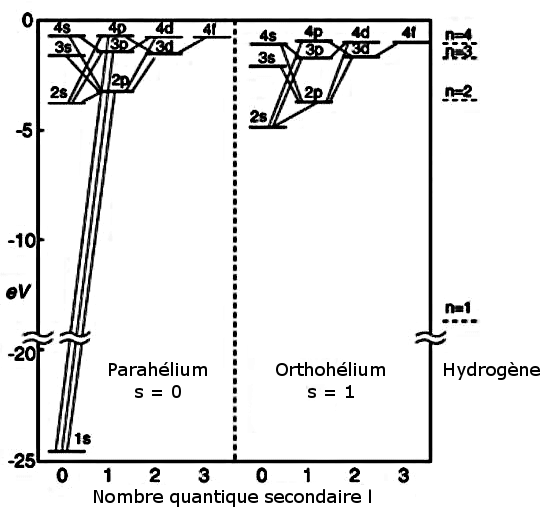
\includegraphics[scale=.7]{chimiePC/atomes/helium.png}
        \caption{Niveaux énergétiques de l'hélium comparés à ceux de l'hydrogène}
    \end{figure}
    
\end{EnvUplevel}
    \question Préciser ce que signifie $s= 0$ et $s = 1$.
    
    \question Représenter par deux diagrammes énergétiques la configuration électronique fondamentale du parahélium et de l'orthohélium. Pourquoi le l'orthohélium n'a pas de niveau 1s sur le schéma ? \'Enoncer la règle illustrée ici.
    \question Comparer les niveaux d'énergie 1s du parahélium et de l'hydrogène et expliquer cette différence.
    \question Représenter les niveaux énergétique des sous-couches de l'hydrogène pour $n\leqslant 3$.
    \question Comparer les les niveaux d'énergie des sous-couches de $n=2$ entre le parahélium et l'hydrogène. Comment s'appelle ce phénomène ?
    \questionbonus Pourquoi ce phénomène n'est pas présent dans l'hydrogène ?
    \question Commenter (sans expliquer) l'ordre des sous-couches $n=3$ et $n=4$ dans le parahélium. \'Enoncer la règle violée.
    \question Comment qualifier les niveaux énergétiques des orbitales atomiques au sein d'une même sous-couche ?
    \question Retrouver la formule donnant le nombre d'orbitales atomiques et le nombre maximal d'électrons dans une couche donnée.
    \question Comparer les les niveaux d'énergie des sous-couches de $n=2$ entre le parahélium et l'orthohélium. \'Enoncer la règle de remplissage illustrée ici ?
    
\end{questions}
\end{exercise}